\section{Drag on the actuator disks}

The measured drag and the calculated drag coefficients related to the produced \gls{AD}s have been studied. The solid disk, used as a reference case, produced the drag seen in figure \ref{Fig:SolidDrag} and the drag coefficient seen in figure \ref{Fig:SolidCD}. There seems to be a deviation of the drag coefficient at $Re \approx 3*10^4$, however, due to limited time and the fact that the solid disk was far from comparable to the rotating models, the measurements were not redone. Further, the drag and the drag coefficient for the two types of disks with 60\% solidity can be seen in figure \ref{Fig:SixtyDrag} and \ref{Fig:SixtyCD}, respectively. 


%For all three disks, the drag is seen to increase with increasing wind velocity, as one would expect. The average drag coefficient and the standard deviation is presented in table \ref{tab:AvgCD}.


\begin{figure} 
    \centering
    \begin{subfigure}[b]{0.45\linewidth}
        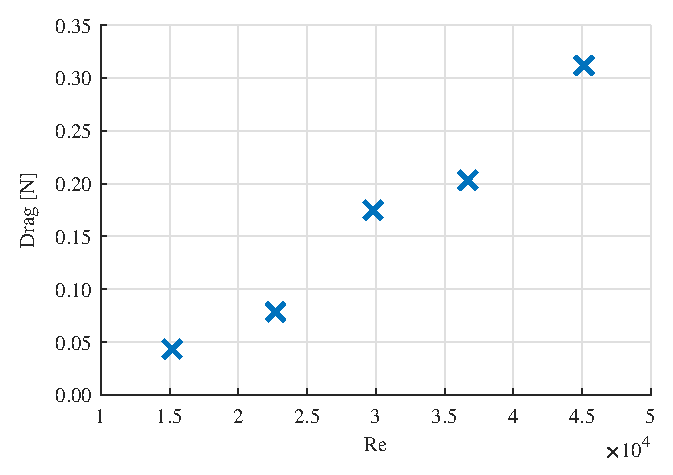
\includegraphics[width=\textwidth]{0_Images/SolidDragRe.eps}
        \caption{The drag.}
        \label{Fig:SolidDrag}
    \end{subfigure}
    ~
    \begin{subfigure}[b]{0.45\linewidth}
        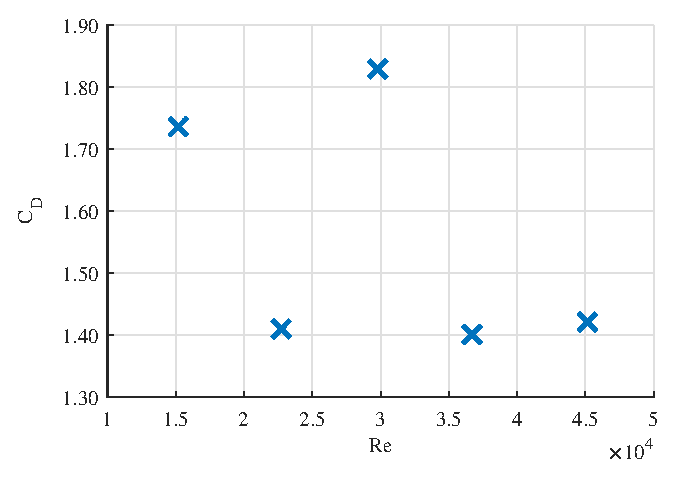
\includegraphics[width=\textwidth]{0_Images/SolidCDRe.eps}
        \caption{The drag coefficient.}
        \label{Fig:SolidCD}
    \end{subfigure}
    \caption{Using the solid disk.}
    \label{fig:SolidDisk}
\end{figure}


\begin{figure} 
    \centering
    \begin{subfigure}[b]{0.45\linewidth}
        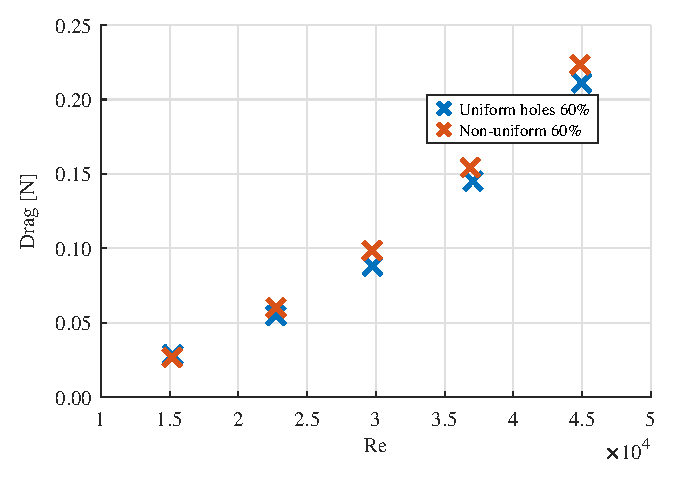
\includegraphics[width=\textwidth]{0_Images/SixtyDragRe.eps}
        \caption{The drag.}
        \label{Fig:SixtyDrag}
    \end{subfigure}
    ~
    \begin{subfigure}[b]{0.45\linewidth}
        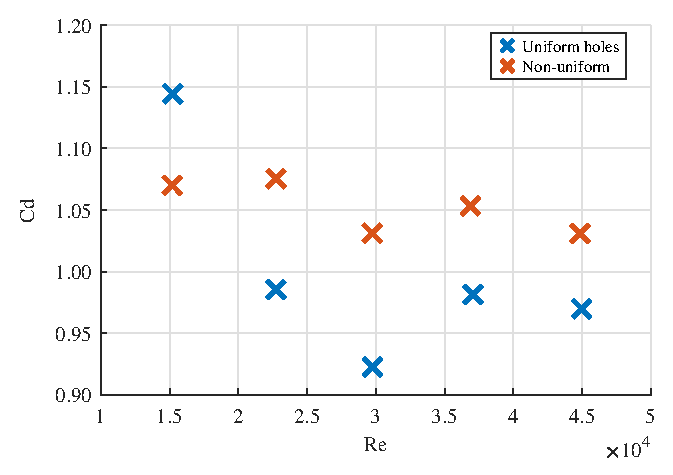
\includegraphics[width=\textwidth]{0_Images/SixtyCDRe.eps}
        \caption{The drag coefficient.}
        \label{Fig:SixtyCD}
    \end{subfigure}
    \caption{Using the disks with 60\% solidity.}
    \label{fig:SixtyDisk}
\end{figure}


The drag for the disks with 40\% and 35\% solidity were plotted in figure \ref{fig:FortyDrag}, and the drag coefficient for the same disks were plotted in figure \ref{fig:FortyCD}. As these disks produced a drag fairly close to the average drag of the \gls{RWTM}s, the average drag and drag coefficient representing the rotating models is also included in the plots, to ease the comparison. 


\begin{figure}
    \centering
    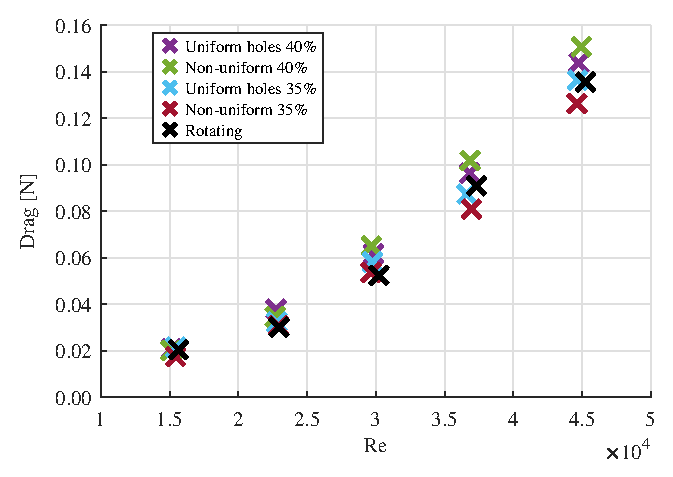
\includegraphics[width=0.8\linewidth]{0_Images/FortyDragRe.eps}
    \caption{The drag for the disks with 40\% and 35\% solidity, compared to the average drag coefficient of the rotating disks.}
    \label{fig:FortyDrag}
\end{figure}

\begin{figure}
    \centering
    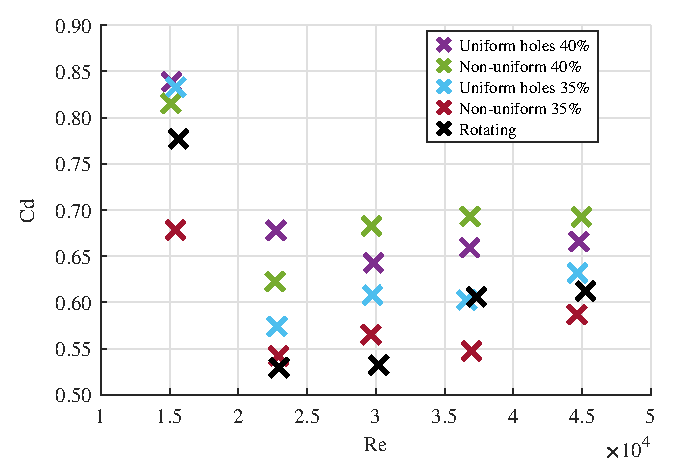
\includegraphics[width=0.8\linewidth]{0_Images/FortyCDRe.eps}
    \caption{The drag coefficient for the disks with 40\% and 35\% solidity, compared to the average drag coefficient of the rotating disks.}
    \label{fig:FortyCD}
\end{figure}


Some general trends can be observed from these graphs. For all the \gls{AD} and \gls{RWTM} measurements, the drag is seen to increase with increasing Re, as one would expect. Another trend that can readily be seen, is that the drag coefficient increases with increasing solidity. This coincides with what has been found in the literature. Lignarolo et al (2016) \cite{Lignarolo2016} presented a comparison between different drag coefficients as a function of solidity, based on the results presented in six different papers. Compared, the \gls{AD}s used in this current study results in a slightly higher drag coefficient for all the solidities. This can be caused by differences in inflow conditions, such as inflow turbulence, or be due to the models being placed in the boundary layer in this study, in contrast to most cases in literature where the hub is in the free stream flow. However, Lignarolo et al also concludes that the drag coefficient seems to be approximately linearly decreasing with decreasing solidity, which is the case with the current measurements as well. 
 % According to this, a solidity of 60\% results in a Cd of around 0.9, a solidity of 40\% results in a Cd between 0.5 and 0.6, and a 35\% solidity results in a Cd between 0.4 and 0.5.

For all the different \gls{AD}s and for the \gls{RWTM}s, the drag coefficient corresponding to $Re \approx 1.5*10^4$ is significantly higher than for the other Reynolds numbers, while the drag coefficient related to the other four Reynolds numbers generally seem to concentrate around some mean value. This deviation at $Re \approx 1.5*10^4$ does not appear in the experiments of Blackmore et al (2013) \cite{Blackmore2013}, who used the same range of Re as in the present study. Thus, the deviation is most likely due to measurement noise. When studying the standard deviation for each 60 \si{\s} measurement, the standard deviation is always between 0.011 and 0.015, independent of which disk is being studied, showing that this is probably the size of the measurement noise related to the transducer and electrical equipment. The drag force at such a low velocity will be quite small, and it seems that the measurement noise is larger than the actual drag and interfering with the measurements. Additionally, it should be pointed out that the drag coefficient at low velocities is much more sensitive to small changes in drag compared to at higher velocities, resulting from equation \ref{Eq:Cd}. However, this result will not have any significant impact on the future work, as the future work will focus around Reynolds numbers higher than $Re \approx 1.5*10^4$ .

%the electrical noise as the signal passes from the force plate, through the amplifier and the lowpass filter. The drag force at such a low velocity will be quite small. 


Looking at figure \ref{fig:FortyCD}, the \gls{spider} with 35\% solidity and the \gls{holes} with 35\% solidity seem to best match the drag of the rotating model. To study this further, the average drag coefficient over the four Reynolds numbers where the measurements already seem to gather around some mean, is calculated, and presented in table \ref{tab:AvgCD}. The standard deviation is also included, as well as the average Cd and the standard deviation for the 40\% \gls{AD}s. If one assumes that the Cd corresponding to the rotating model is correct, and that the \gls{AD}s have a Gaussian distribution, it can be seen that the standard deviation of both disks with 35\% solidity covers the rotating Cd value, while neither of the 40\% solidity disks do. Thus, it is concluded that the disks with 35\% solidity is the best match, and based on the averages it seems that the \gls{spider} with 35\% solidity is the closest match, while the \gls{holes} with 35\% solidity is the second closest.


\begin{table}
    \centering
    \begin{tabular}{l c c r}
         Disk type & Average Cd & Cd standard deviation \\
         \hline
         Rotating average & 0.570 & 0.082 \\
         %Solid & 1.515 \\
         %Uniform holes, 60\% & 0.965 \\
         %Non-uniform, 60\% & 1.048\\
         Uniform holes, 40\% & 0.662 & 0.053 \\
         Non-uniform, 40\% & 0.673 & 0.057 \\
         Uniform holes, 35\% & 0.604 & 0.051 \\
         Non-uniform, 35\% & 0.560 & 0.051 \\
    \end{tabular}
    \caption{Average Cd for the rotating model and the disks with 35\% solidity.}
    \label{tab:AvgCD}
\end{table}



%Assuming that rotating is correct - p verdi, gitt normalfordelig med sd og mean, hva er sanns for at denne disken ligger innenfor. vil også si at 40 og rot ikke passer 
%viser også at det er mulig å finne en nøytakig 
%+- SD




%for last one, 0.5843 without drift 



%Which SD is relevant? I have the ones for each measurement... But maybe the ones for Cd also? 

%\section{Noise and other possible sources of error}

%\begin{figure}[h!]
%    \centering
%    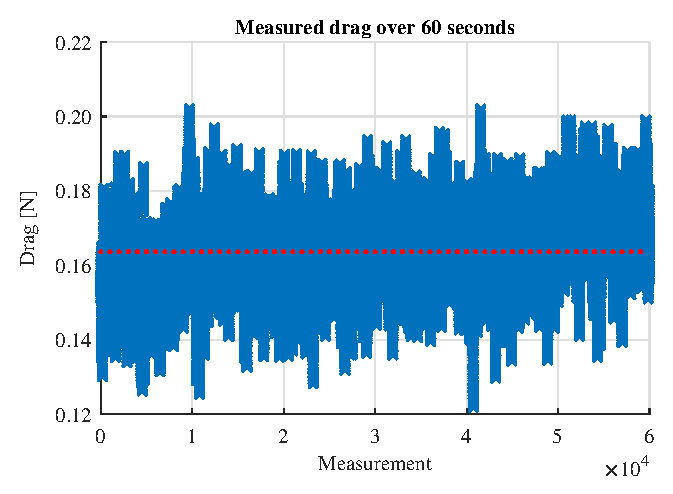
\includegraphics[width=\linewidth]{0_Images/NoiseFirst.eps}
%    \caption{The drag for the solid disk at 5 m/s.}
%    \label{fig:Noise}
%\end{figure}

%Figure \ref{fig:Noise} shows each measured drag value at a sampling rate of 1000 Hz over the course of 60 seconds. The measured drag varies with a 0.012, compared to an average of 0.1636. This means that the noise is of one order less that the average. 

%This noise may both be related to measurement noise in the force plate, and electrical noise as the signal passes from the force plate, through the amplifier and the lowpass filter. 
%It is still a reasonable assumption that the measurements have a Gaussian distribution and that the average drag is representative. 

%It can also be seen that the \gls{spider} produces a slightly higher drag compared to the \gls{holes} with the same solidity for 60\% and 40\% solidity. The same trend can not be seen at 35\% solidity, where \gls{holes} seem to produce the largest drag. However, as mentioned, the \gls{holes} design with 35\% solidity was created in a slightly different way than those with 40\% and 60\% solidity, and they may not be exactly comparable. 

An additional remark that can be made is that there does not seem to be a clear trend regarding the drag produced when using the \gls{spider} design compared to the drag produced when using the \gls{holes} design, in terms of one design consistently producing a larger or a smaller drag than the other. 

%the drag coefficient when using the \gls{spider} design compared to when using the \gls{holes} design. 


%Error, standard deviation 

%why do we get the results that we get? 

%- Adjusting for drift 
%- statistikk arument 
%- usikkerhet



